\documentclass[fleqn]{beamer}
\usepackage{handout}
\definecolor{Green}{RGB}{0,100,0}
\title{The impact of daily diet and exercise on weight}
\author{\href{mailto: korenson@cs.ccu.edu.tw}{Ren-Song Ko}, \href{mailto: hwshuo111u@cs.ccu.edu.tw}{Wen-Shou Hsu}, and  \href{mailto: stchi111u@cs.ccu.edu.tw}{Tzu-Chi Hsiao}}
\date{}
\begin{document}
\fontspec{Times New Roman}  
\begin{frame}
\titlepage
\begin{center}
Official website is available \href{https://www2.cs.ccu.edu.tw/~stchi111u/project/}{here}. \\
Source code is available \href{https://www2.cs.ccu.edu.tw/~stchi111u/project/下載/index.html}{here}.
\end{center}
\begin{figure}[h]
\centering

\includegraphics[width=0.10\textwidth]{logo.png}
\end{figure}
\begin{center}
Floor One, Innovation Building \\
National Chung Cheng University, Chiayi county, Taiwan
\end{center}
\end{frame}
\begin{frame}
\frametitle{Outline}
\begin{itemize}
\item Introduction \\
\item Tools for develop model \\
\item Results \\
\item Conclusion
\end{itemize}
\end{frame}
\begin{frame}
\frametitle{Outline}
\begin{itemize}
\item Introduction \\
\item \textcolor{gray}{Tools for develop model} \\
\item \textcolor{gray}{Results} \\
\item \textcolor{gray}{Conclusion}
\end{itemize}
\end{frame}
\begin{frame}
\frametitle{Introduction}
\begin{itemize}
\item People emphasize their health and strengthen it by exercising at the gym, in the park, or even at home. \\
\item We aim to establish a website to help them check whether their \alert{healthy} is normal. \\
\item Given their \textcolor{blue}{age, gender, height, weight, eating habits, activity level, goal, daily calories} and \textcolor{blue}{after days}. \\
\item Displays result with suggestions and amounts of each nutrient in a histogram. 
\end{itemize}
\end{frame}
\begin{frame}
\frametitle{Outline}
\begin{itemize}
\item \textcolor{gray}{Introduction} \\
\item Tools for develop model \\
\item \textcolor{gray}{Results} \\
\item \textcolor{gray}{Conclusion}
\end{itemize}
\end{frame}
\begin{frame}
\frametitle{Tools for develop model}
\begin{itemize}
\item Programming Language via CSS, HTML, JavaScript and Python. \\
\item Data transmitting via Flask. \\
\item Aesthetic via JavaScript.
\end{itemize}
\end{frame}
\begin{frame}
\frametitle{Outline}
\begin{itemize}
\item \textcolor{gray}{Introduction} \\
\item \textcolor{gray}{Tools for develop model} \\
\item Results \\
\item \textcolor{gray}{Conclusion} \\
\end{itemize}
\end{frame}
\begin{frame}
\frametitle{Results}
\begin{minipage}[t]{0.48\textwidth}
\setbeamercolor{block title}{bg=red,fg=white}
\setbeamerfont{block title}{size=\normalsize}
\setbeamerfont{block body}{size=\normalsize}
\begin{block}{Our anticipate}
\setbeamercolor{itemize item}{fg=red}
\begin{itemize}
\item Accurately calculate the actual results using BMR, TDEE, and so on. \\
\item Provide a histogram to show the amounts of each nutrient. 
\end{itemize}
\end{block}
\end{minipage}
\hfill
\begin{minipage}[t]{0.48\textwidth}
\setbeamerfont{block title}{size=\normalsize}
\setbeamerfont{block body}{size=\normalsize}
\setbeamercolor{block title}{bg=Green,fg=white}
\begin{block}{Our website anticipate}
\begin{itemize}
\setbeamercolor{itemize item}{fg=Green}
\item Suggestion.
\item A histogram displays each nutrient.
\end{itemize}
\end{block}
\end{minipage}
\end{frame}
\begin{frame}{Results (Continued)}
\begin{figure}[h]
\centering
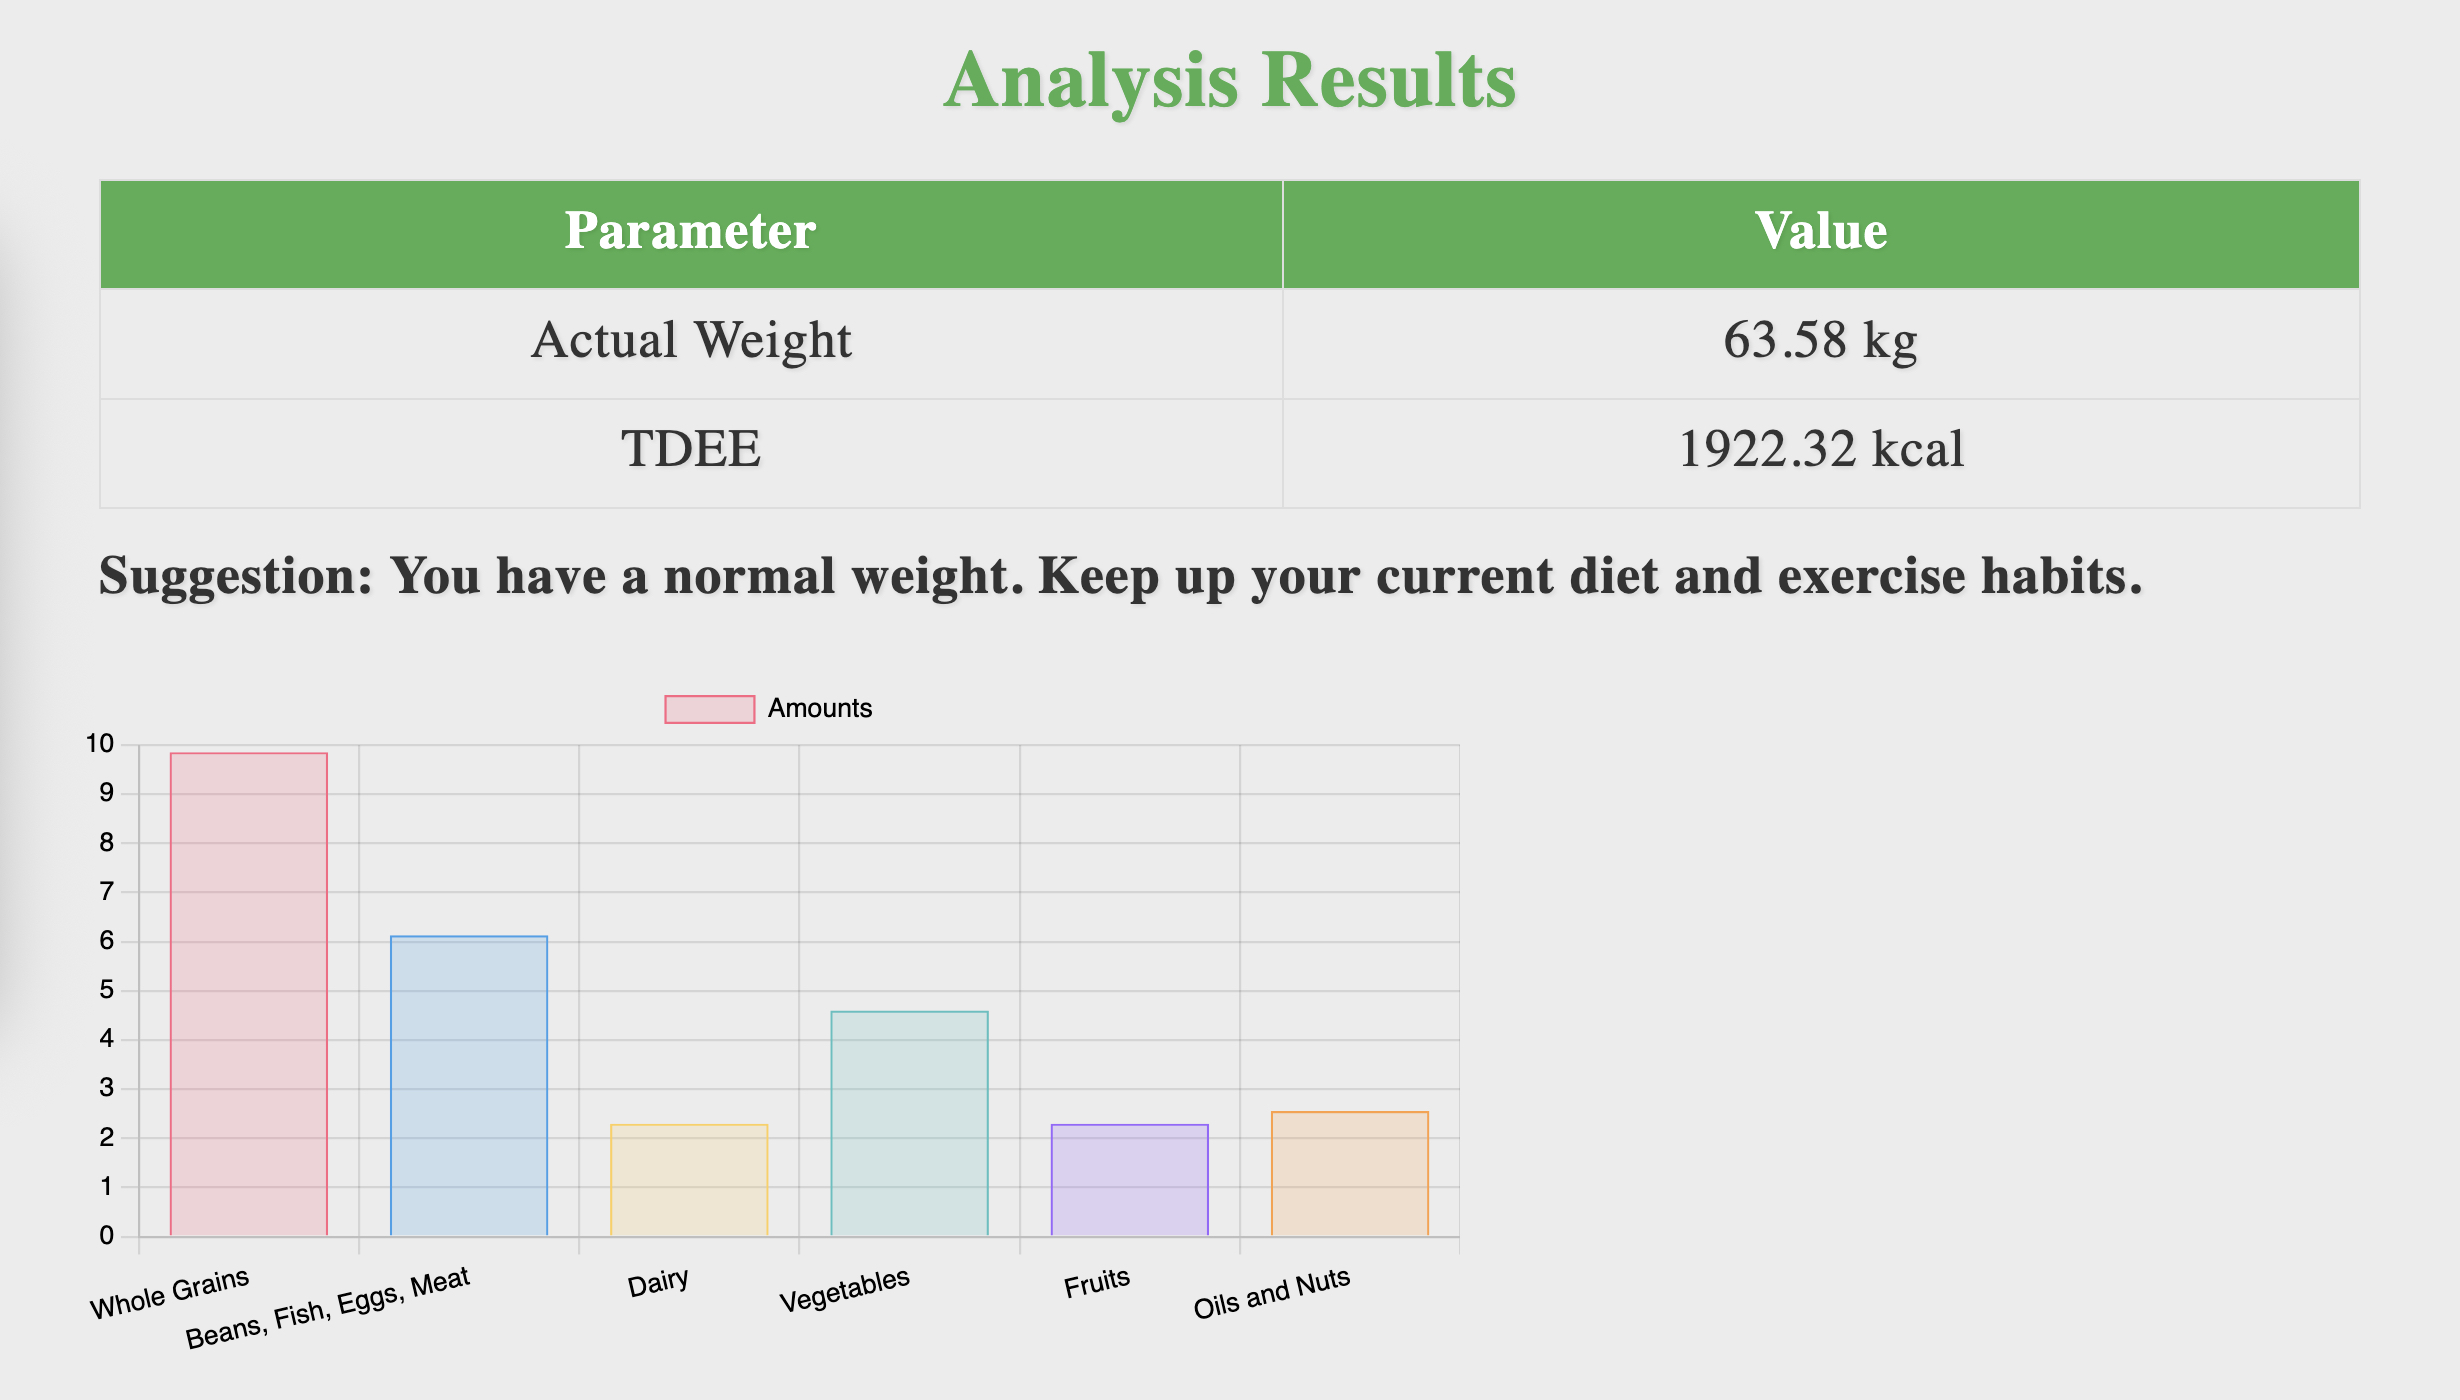
\includegraphics[width=\textwidth]{Example.png}
\end{figure}
\centering
Figure I. Results of entering data.
\end{frame}
\begin{frame}{Results (Continued)}
\vspace{2em}
\sloppy
\renewcommand{\arraystretch}{1.35}
\centering
\begin{tabular}{|c|c|c|c|c|}
\hline
Sedentary & Light & Moderate & Active & Very active \\
\hline
1.2 & 1.375 & 1.55 & 1.725 & 1.9 \\
\hline
\end{tabular}
\vspace{1em} \\
Table I. Consume calories from the exercise. 
\vspace{1em} \\
\begin{tabular}{|c|c|c|c|}
\hline
Vegetarian & Meat & Lacto ovo vegetarian & Balanced \\
\hline
1800 & 2500 & 2200 & 2000 \\
\hline
\end{tabular}
\vspace{1em} \\
Table II. Consume calories from the daily diet. 
\vspace{1em} \\
\end{frame}
\begin{frame}{Results (Continued)}
\sloppy
\begin{align*}
\text{Male's BMR} &= (9.99 \times \text{weight}) + (6.25 \times \text{height}) \\
&\quad - (4.92 \times \text{age}) + (166 \times \text{gender} - 161) \\
\end{align*}
\begin{align*}
\text{Female's BMR} &= (9.99 \times \text{weight}) + (6.25 \times \text{height}) \\
&\quad - (4.92 \times \text{age}) + (166 \times \text{gender} - 161)
\end{align*}
\end{frame}
\begin{frame}{Results (Continued)}
\sloppy
\begin{align*}
\text{Each day} = \text{BMR} \times \text{Activity}
\end{align*}
\begin{align*}
\text{Calorie deficit} = \text{Intake} - \text{Calories per day}
\end{align*}
\begin{align*}
\text{Weight changes} = \frac{\text{Calorie deficit}}{7700} 
\end{align*}
\begin{align*}
\text{Actual weight}= \text{Weight} + \text{Weight changes} \times \text{After days}
\end{align*}
\begin{align*}
\text{BMI} = \frac{\text{Actual Weight}}{\text{Height}^2}
\end{align*}
\end{frame}
\begin{frame}
\frametitle{Outline}
\begin{itemize}
\item \textcolor{gray}{Introduction} \\
\item \textcolor{gray}{Tools for develop model} \\
\item \textcolor{gray}{Results} \\
\item Conclusion
\end{itemize}
\end{frame}
\begin{frame}
\frametitle{Conclusion}
\begin{itemize}
\item Using precise tools to calculate the actual weight, ensuring that users receive accurate and reliable measurements for better health management. \\
\pause
\item Providing accurate options for computation, allowing users to input various parameters and receive tailored recommendations based on their unique needs. \\
\pause
\item We learned fundamental front-end and back-end development, including figure display using JavaScript and Python, to develop an application that seamlessly integrates user data and visualizes results effectively.
\end{itemize}
\end{frame}
\begin{frame}{Acknowledgment}
\begin{block}{}
\normalsize
\setbeamerfont{block title}{size=\normalsize}
\setbeamerfont{block body}{size=\normalsize}
\setbeamercolor{itemize item}{fg=Blue}
\begin{itemize}
\setbeamerfont{itemize}{size=\small}
\item Ren-Song Ko
\item Wen-Shuo Hsu
\item Tzu-Chi Hsiao
\end{itemize}
\end{block}
\vspace{1em}
\begin{block}{}
\normalsize
\setbeamerfont{block title}{size=\normalsize}
\setbeamerfont{block body}{size=\normalsize}
\begin{center}
\setbeamerfont{itemize}{size=\small}
\textcolor{purple}{Thank you for listening! We wish you a pleasant day.}
\end{center}
\end{block}
\end{frame}
\end{document}
